\section{Exercise 6}
Cho mạch sau. Áp dụng kiến thức bạn đã học để biến nó thành một dạng khác mà bạn có thể tìm thấy điện trở tương đương \(R_{ab}\) dễ dàng hơn. Tiếp theo, tìm
giá trị của dòng điện \(i\) qua mạch và thực hiện mô phỏng để kiểm tra.
\begin{figure}[!htbp]
    \centering
    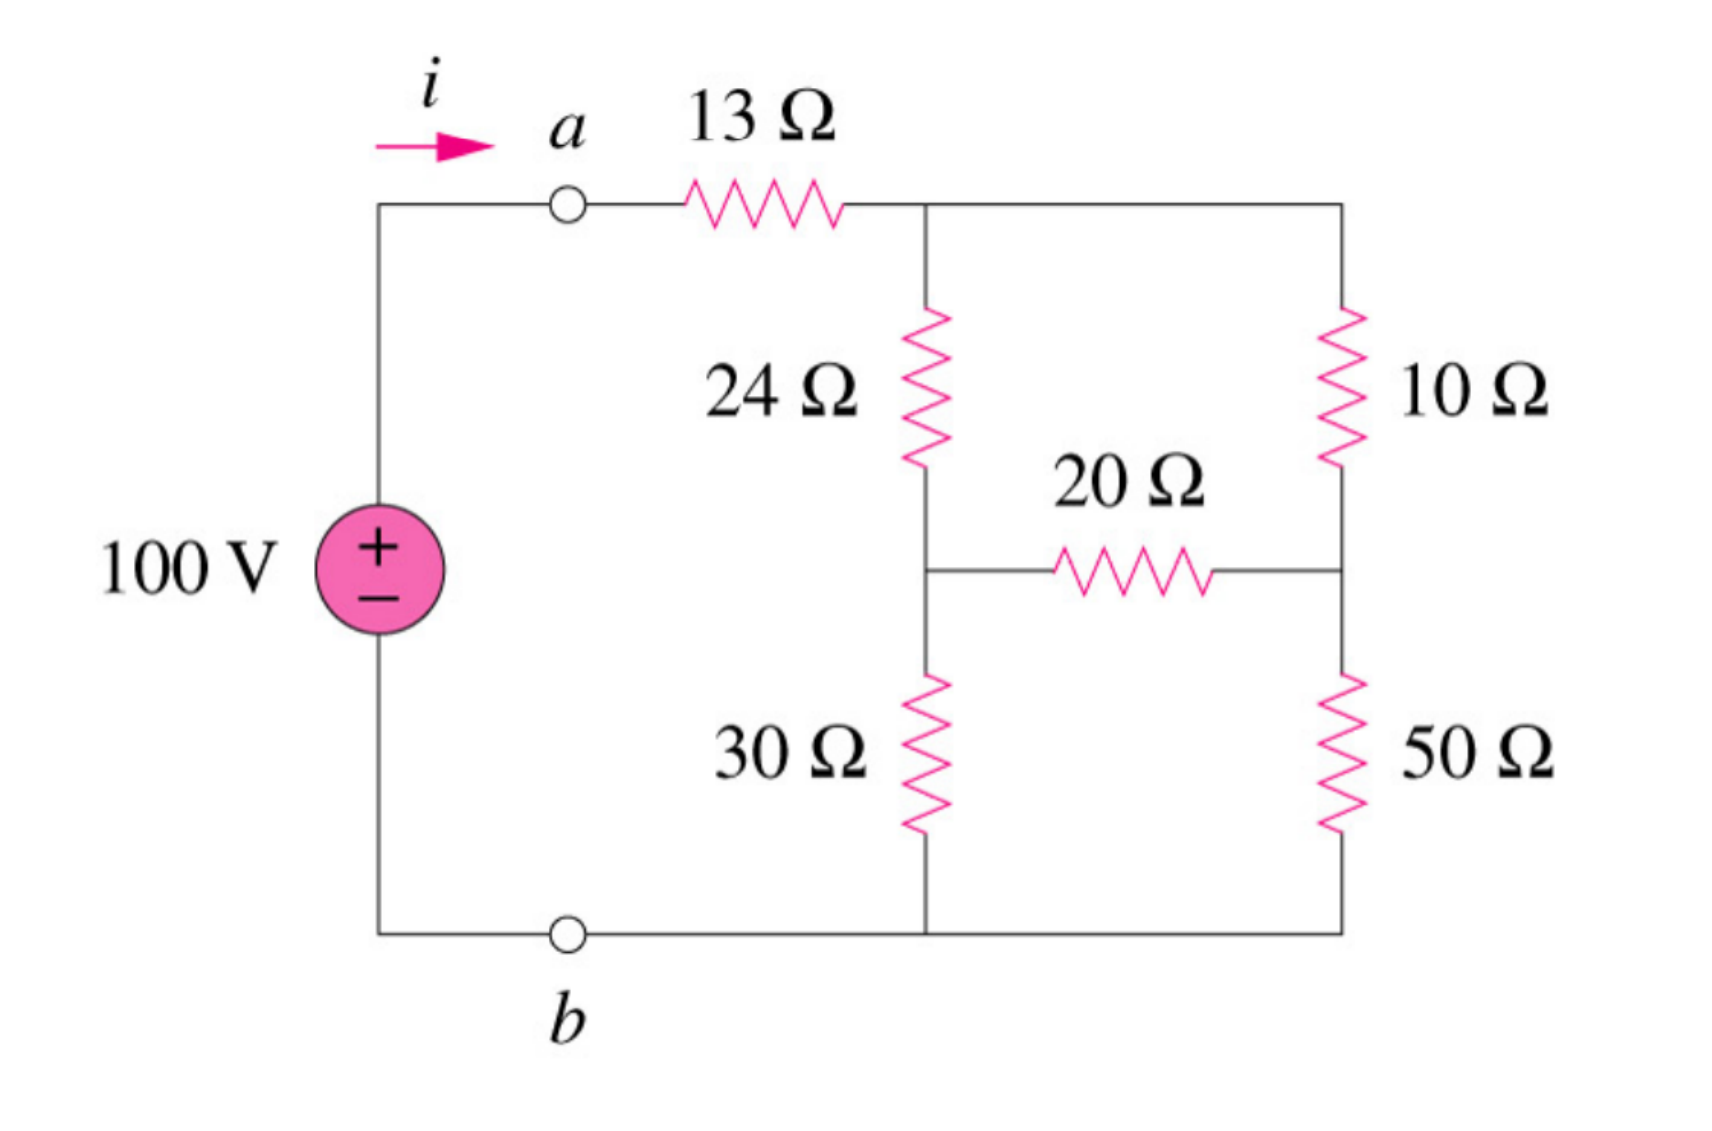
\includegraphics[width=0.7\textwidth]{graphics/ex6/f1.png}
    \caption{Biến đổi mạch điện rồi tìm điện trở tương đương \(R_{ab}\) và cường độ dòng điện
    \(i\) thông qua mạch điện.}
    \end{figure}
\subsection{Chuyển đổi mạch}
\begin{figure}[!htbp]
    \centering
    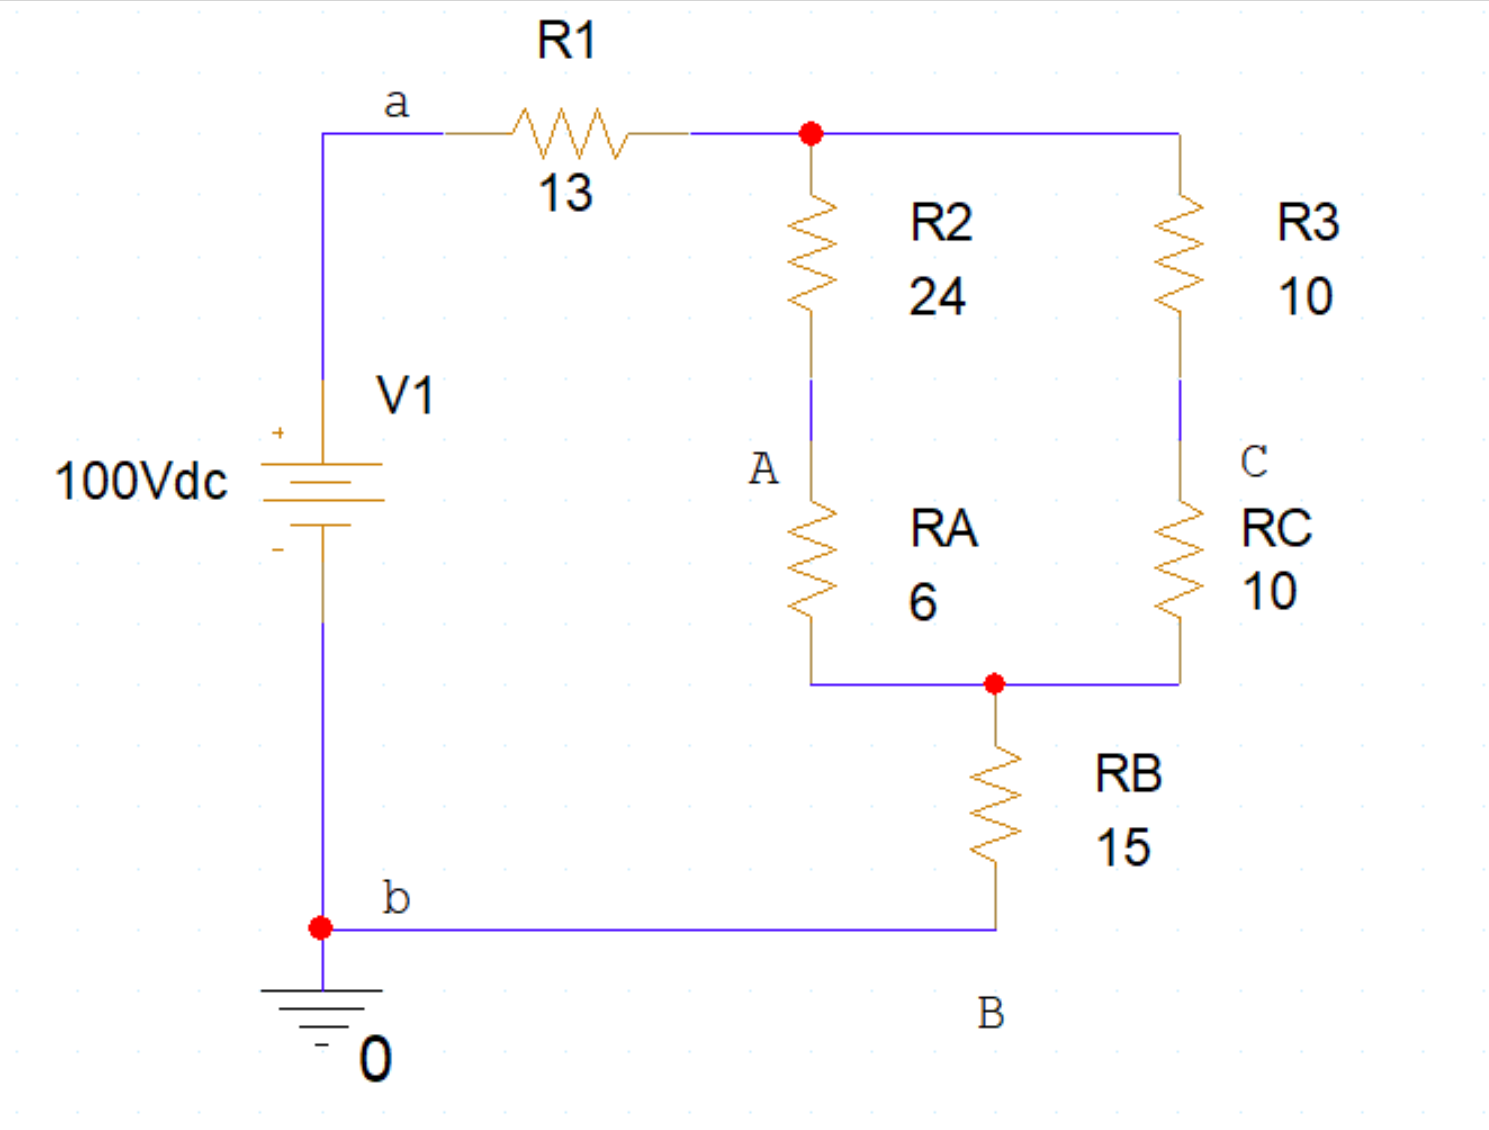
\includegraphics[width=0.7\textwidth]{graphics/ex6/f2.png}
    \caption{Chuyển đoạn mạch delta (\(R_a, R_b, R_c\)) sang mạch wye (\(R_A, R_B, R_C\))}
    \end{figure}
\begin{center}
    \textbf{Tính Toán và giải thích}\\
    Các phương trình biến đổi từ delta sang wye:\\
    \(R_A = \dfrac{R_b*R_c}{R_a + R_b + R_c} = \dfrac{20*30}{20 + 30 + 50} = 6 \Omega\)\\
    \(R_B = \dfrac{R_a*R_c}{R_a + R_b + R_c} = \dfrac{50*30}{20 + 30 + 50} = 15 \Omega\)\\
    \(R_C = \dfrac{R_b*R_a}{R_a + R_b + R_c} = \dfrac{20*50}{20 + 30 + 50} = 10 \Omega\)\\
\end{center}
\begin{figure}[!htbp]
    \centering
    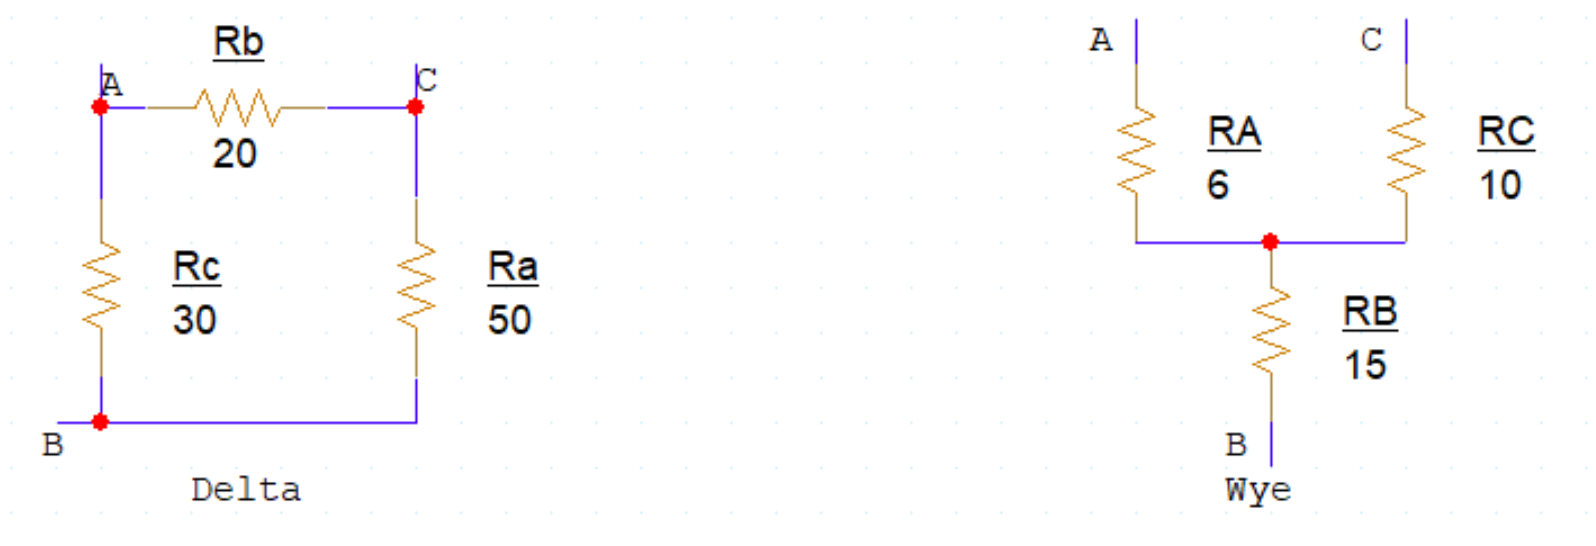
\includegraphics[width=1\textwidth]{graphics/ex6/f7.png}
    \caption{Chuyển đoạn mạch delta sang mạch wye như sau}
    \end{figure}
    
    \begin{figure}[!htbp]
    \centering
    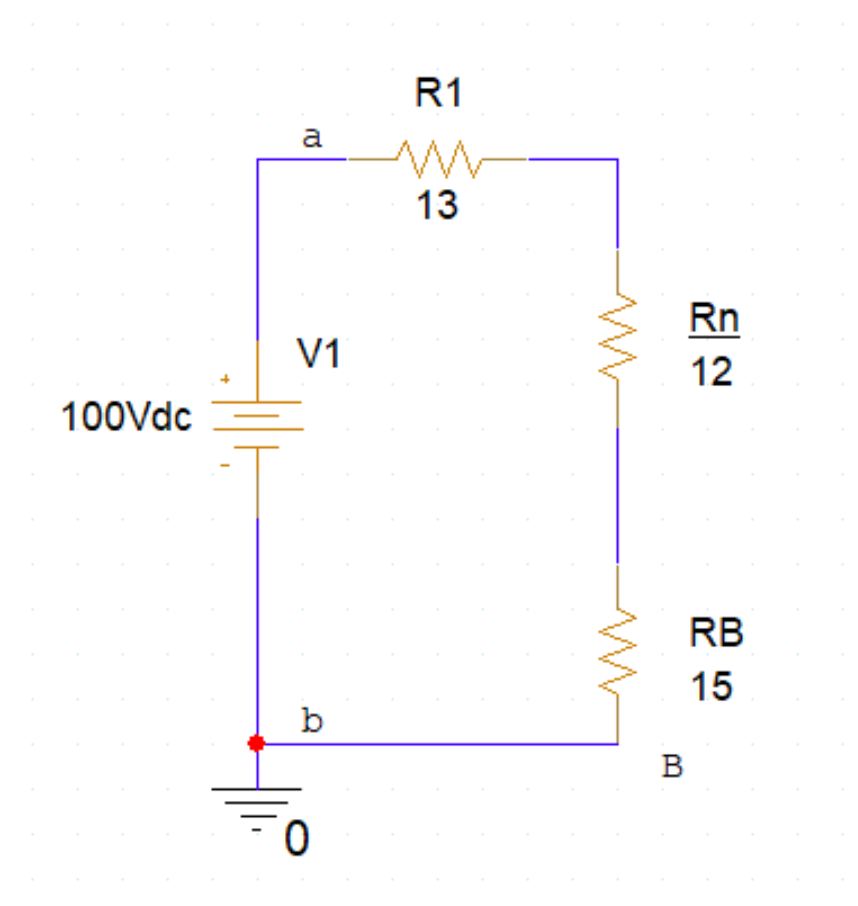
\includegraphics[width=0.6\textwidth]{graphics/ex6/f3.png}
    \caption{Chuyển mạch chứa \((R_2 nt R_A) // (R_3 nt R_C)\) thành \(R_n\)}
    \end{figure}
    \begin{center}
        \textbf{Tính Toán và giải thích}\\
        \((R_2 nt R_A) // (R_3 nt R_C) \rightarrow \dfrac{1}{R_n} = \dfrac{1}{R_2 + R_A} + \dfrac{1}{R_3 + R_C} = \dfrac{1}{24 + 6} + \dfrac{1}{10+10} = \dfrac{1}{12} \rightarrow R_n = 12 \Omega \)
    \end{center}
    \subsection{Tính toán}
    \begin{itemize}
        \item Do \(R_1, R_n, R_B\) nối tiếp nhau \(\rightarrow \) \(R_{ab} = R_1 + R_n + R_B = 13 + 12 + 15 = 40 \Omega \)
        \item Áp dụng định luật Ohm, \(i = \dfrac{U}{R_{ab}} = \dfrac{100}{40} = 2,5 A\)
    \end{itemize}
    \subsection{Mô phỏng}
    \textbf{Hình kết quả mô phỏng}
    \begin{figure}[!htbp]
    \centering
    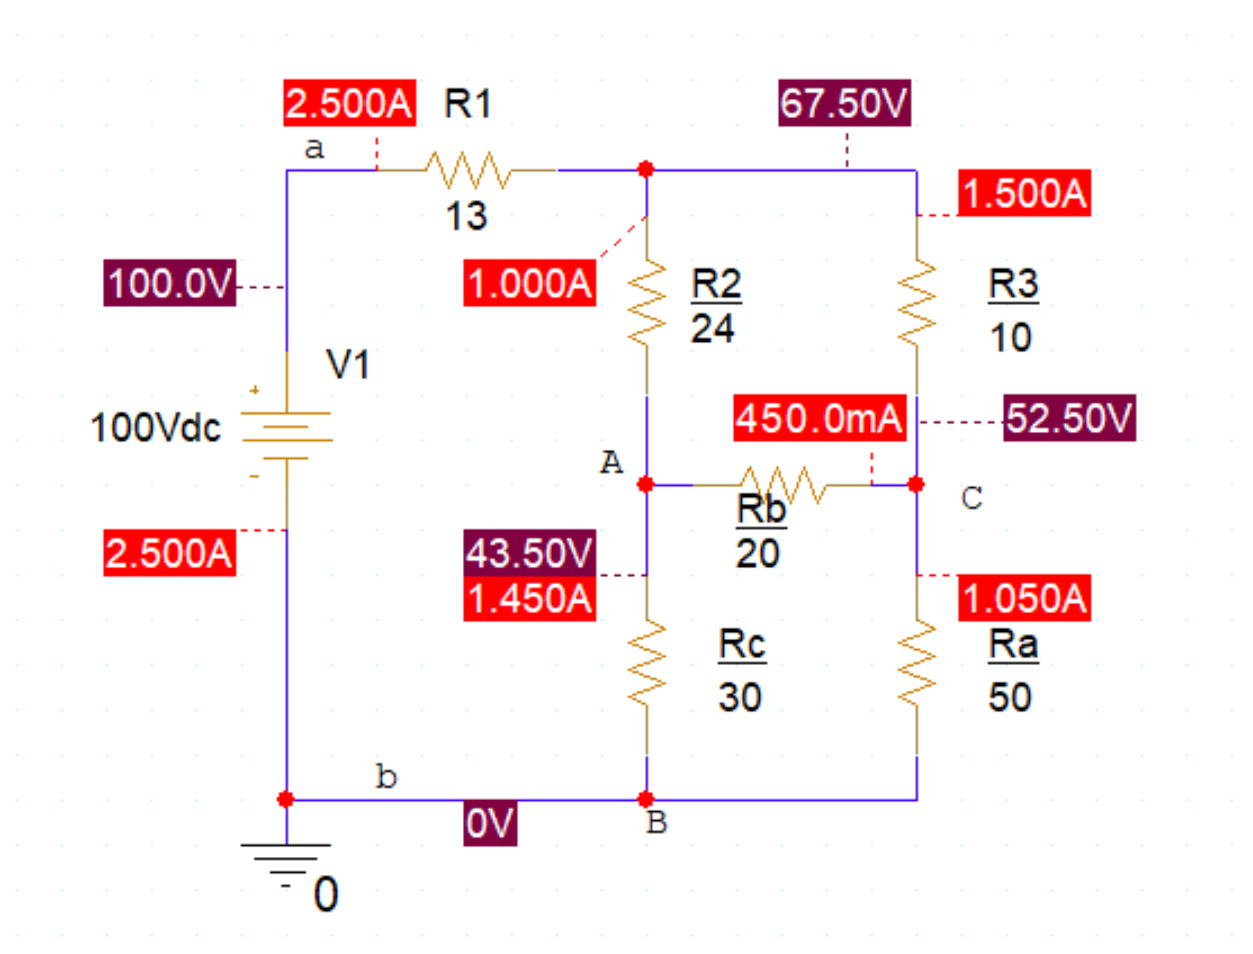
\includegraphics[width=0.8\textwidth]{graphics/ex6/f5.png}
    \caption{Mạch ban đầu}
    \end{figure}
    \begin{figure}[!htbp]
    \centering
    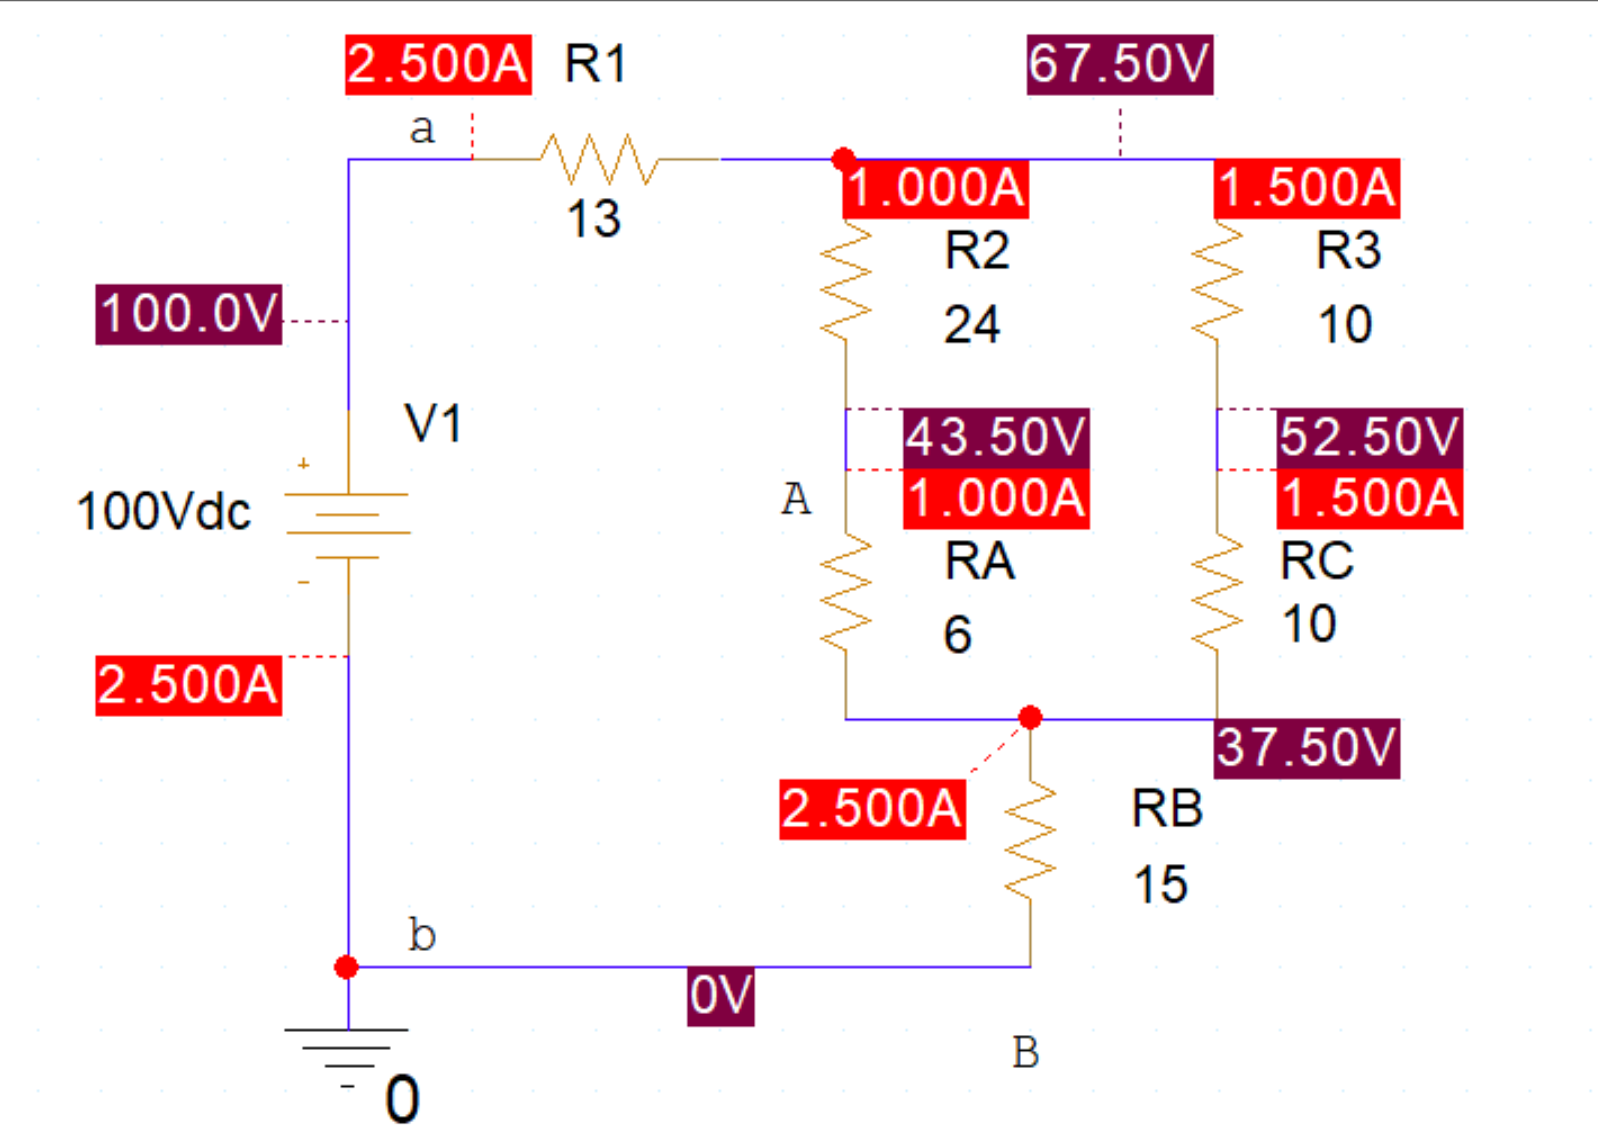
\includegraphics[width=0.8\textwidth]{graphics/ex6/f6.png}
    \caption{Mạch biến đổi delta-wye}
    \end{figure}
    \begin{figure}[!htbp]
        \centering
        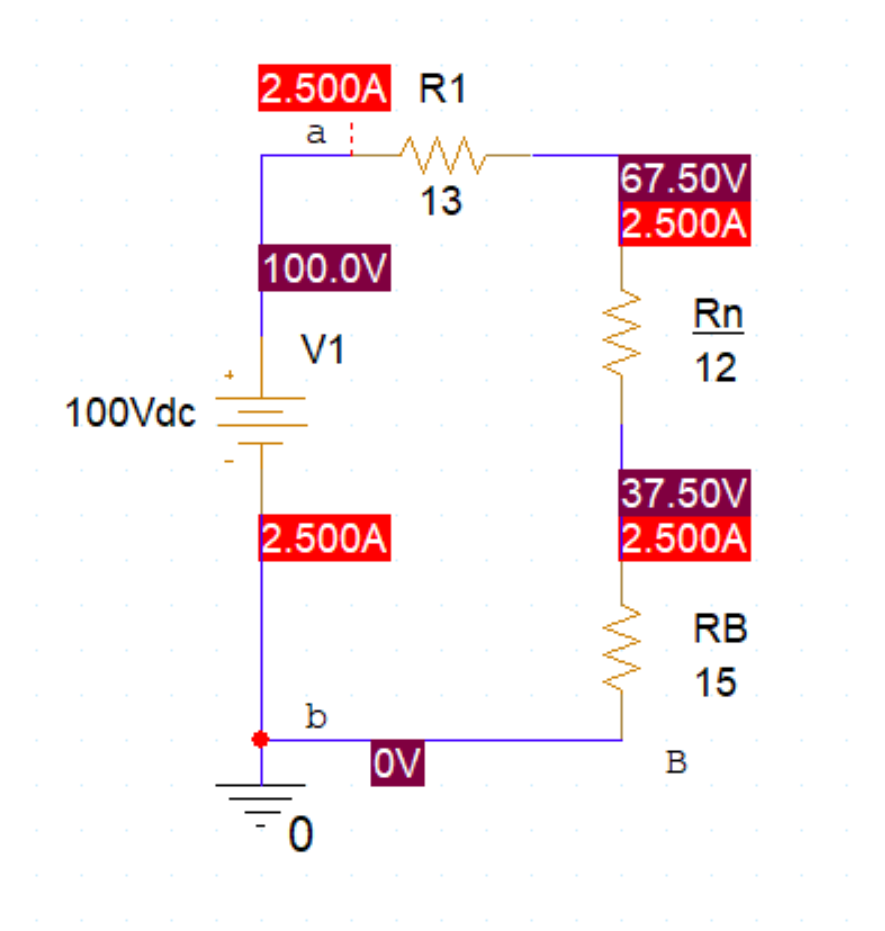
\includegraphics[width=0.6\textwidth]{graphics/ex6/f4.png}
        \caption{Mạch tương đương}
        \end{figure}

    
